%% IEEE Access LaTeX Template
%% Title: AI Finance Assistant with Risk Analysis and Deal Detection
%% Compile with: pdflatex -> bibtex -> pdflatex -> pdflatex

\documentclass[]{IEEEtran}

\usepackage{cite}
\usepackage{amsmath,amssymb,amsfonts}
\usepackage{algorithmic}
\usepackage{graphicx}
\usepackage{textcomp}
\usepackage{xcolor}
\usepackage{booktabs}
\usepackage{multirow}
\usepackage{url}
\usepackage{hyperref}
\usepackage{float}
\usepackage{array}
\usepackage{tabularx}
\usepackage{balance}
\usepackage{pgfplots}
\pgfplotsset{compat=1.18}
\usepgfplotslibrary{colorbrewer}
\usetikzlibrary{patterns}

\def\BibTeX{{\rm B\kern-.05em{\sc i\kern-.025em b}\kern-.08em
    T\kern-.1667em\lower.7ex\hbox{E}\kern-.125emX}}

\begin{document}

\title{AI Finance Assistant with Risk Analysis and Deal Detection: An Integrated Architecture Combining FinGuard and DealDetective}

\author{
\IEEEauthorblockN{Hema Surya}
\IEEEauthorblockA{
\textit{Department of Computer Science and Engineering} \\
\textit{[Institution Name]}\\
[City, Country] \\
hemasurya106@email.com}
}

\maketitle

\begin{abstract}
Personal financial decision-making is increasingly challenged by information overload, impulse spending, and the difficulty of identifying genuine value in a dynamic e-commerce landscape. This paper presents an integrated AI-driven financial assistant that combines two complementary subsystems: \textbf{FinGuard}, a personal finance intelligence engine for risk analysis, and \textbf{DealDetective}, an AI-powered product deal finder and price monitoring system. FinGuard employs a staged machine-learning pipeline---encompassing K-Means clustering, Isolation Forest anomaly detection, and a Decision Outcome Learning Engine (DOLE) built on Random Forest---to analyze daily spending behavior and provide actionable risk verdicts. A Gemini 2.5 Flash-powered Text-to-SQL chat interface enables natural-language queries over personal financial data. DealDetective complements this by scraping product listings from major Indian e-commerce platforms (Amazon, Flipkart, Snapdeal), generating 768-dimensional semantic fingerprints using Google's \texttt{text-embedding-004} model stored in a \texttt{pgvector}-enabled PostgreSQL database, offering AI-generated product analysis (jargon decoding, eco-scoring), and sending automated email price alerts. Together, the two systems form a unified pipeline that assists users in both controlling outgoing expenditure and maximizing value in purchasing decisions. Experimental evaluation demonstrates the effectiveness of the full ML pipeline in classifying high-risk spending days, while qualitative assessment validates the accuracy of the deal-detection and product-matching components. The integrated system is implemented as a full-stack application comprising two FastAPI backends, a React frontend for FinGuard, and a React frontend for DealDetective, with a shared PostgreSQL database layer.
\end{abstract}

\begin{IEEEkeywords}
Personal Finance, Anomaly Detection, Machine Learning, Deal Detection, Large Language Models, Gemini API, K-Means Clustering, Isolation Forest, Random Forest, pgvector, Natural Language Processing, Text-to-SQL, Price Monitoring, e-Commerce
\end{IEEEkeywords}

%% ---------------------------------------------------------------
\section{Introduction}
\label{sec:intro}
%% ---------------------------------------------------------------

The rapid proliferation of digital payment systems and e-commerce platforms has created a dual challenge for modern consumers: managing personal expenditure against dynamically shifting spending patterns, and discerning genuine deals from manipulated discount displays. Traditional budgeting tools are predominantly rule-based and fail to adapt to individual behavioral rhythms, while product comparison portals rely on static price snapshots without providing semantic understanding of product value or personalized affordability context.

This work presents an integrated AI Finance Assistant that addresses both dimensions. The system consists of two tightly coupled but independently deployable modules:

\begin{itemize}
    \item \textbf{FinGuard} --- A personal financial intelligence system that tracks daily expenses, classifies spending behavior using unsupervised machine learning, detects anomalous expenditure patterns, simulates future purchase affordability using a burn-rate model, learns from past decision outcomes via a reinforcement-inspired learning engine (DOLE), and supports natural-language financial queries via a Text-to-SQL interface powered by the Gemini LLM.
    
    \item \textbf{DealDetective} --- A product deal intelligence system that extracts real-time product data (price, specifications, images) from Amazon.in, Flipkart, and Snapdeal via a multi-strategy web scraper, computes semantic product fingerprints using Google's embedding model for similarity-based product matching (``Twin Finder''), generates structured AI analysis of product specifications, maintains price history, and delivers automated email alerts when prices drop to user-defined targets.
\end{itemize}

The core contribution of this paper is the description and evaluation of this two-module integrated architecture. By combining outgoing spend risk analysis with incoming purchase opportunity detection, the system provides a holistic view of a user's financial decisions.

The remainder of the paper is organized as follows. Section~\ref{sec:related} reviews related work. Section~\ref{sec:arch} presents the overall system architecture. Section~\ref{sec:methodology} describes the algorithms and models used. Section~\ref{sec:impl} provides implementation details. Section~\ref{sec:results} presents results and analysis. Section~\ref{sec:discussion} discusses findings and limitations, and Section~\ref{sec:conclusion} concludes.

%% ---------------------------------------------------------------
\section{Related Work}
\label{sec:related}
%% ---------------------------------------------------------------

\subsection{AI-Powered Personal Finance}
Personal finance management systems have evolved from simple budgeting apps to ML-driven platforms. Mint \cite{mint2023} and YNAB represent rule-based systems that require manual categorization. Research into automated transaction categorization has applied SVMs \cite{bose2016}, convolutional neural networks \cite{carta2021}, and transformer-based models \cite{yang2022} with increasing accuracy. Anomaly detection in financial transactions has been extensively studied in the context of fraud detection \cite{pozzolo2015}, with Isolation Forest \cite{liu2008} and Autoencoder-based approaches consistently achieving high AUC scores. Our work adapts Isolation Forest to the domain of personal spending pattern analysis, a less-explored application.

\subsection{Behavioral Spending Analysis}
Cluster-based segmentation of consumer spending behavior has been studied using K-Means \cite{wu2019spending} and Gaussian Mixture Models \cite{sharma2021}. Our staged pipeline extends this by adapting the analysis strategy to data maturity: heuristic rules for sparse data (fewer than 15 days), and full ML for mature datasets, a design choice inspired by cold-start mitigation strategies \cite{lika2014}.

\subsection{LLM-Driven Financial Interfaces}
The application of Large Language Models to structured data retrieval via Text-to-SQL \cite{yu2018spider} has gained significant traction. Works such as DINSQL \cite{pourreza2023} and ACT-SQL \cite{zhang2023act} demonstrate LLM capability in generating syntactically and semantically correct queries. Our implementation uses Gemini 2.5 Flash Lite with multi-query decomposition to answer complex financial questions.

\subsection{Product Price Monitoring and Deal Detection}
Web scraping for price tracking has been applied by commercial services (CamelCamelCamel \cite{camel2024}) and studied academically \cite{chen2016product}. Semantic product similarity for ``find similar'' features has been explored using BERT embeddings \cite{devlin2018} and product knowledge graphs \cite{xu2020product}. Our use of pgvector \cite{pgvector2024} for vector similarity search within PostgreSQL offers a practical, unified-database approach compared to dedicated vector databases.

\subsection{Multi-Platform E-Commerce Data Extraction}
Structured data extraction across heterogeneous e-commerce platforms is challenging due to anti-scraping measures and dynamic rendering. Works by \cite{mazloom2022} study platform-specific CSS selector strategies, while \cite{vosecky2019} address JavaScript-rendered content via headless browsers. Our scraper service uses a dual-strategy approach: static \texttt{requests}-based fetching with Playwright fallback.

%% ---------------------------------------------------------------
\section{System Architecture}
\label{sec:arch}
%% ---------------------------------------------------------------

\subsection{Overall Pipeline}

The integrated system operates as a two-backend, two-frontend architecture backed by a shared PostgreSQL instance extended with the \texttt{pgvector} extension. Figure~\ref{fig:arch_overview} illustrates the high-level architecture.

\begin{figure}[H]
    \centering
    % TODO: Replace with actual architecture diagram
    \fbox{\parbox{0.42\textwidth}{\centering \vspace{2cm}
    \textbf{[Figure Placeholder]} \\
    Overall System Architecture Diagram \\
    (FinGuard + DealDetective + User Interaction) \\
    \vspace{2cm}}}
    \caption{High-level architecture of the AI Finance Assistant. The left branch shows the FinGuard pipeline (expense ingestion $\rightarrow$ ML pipeline $\rightarrow$ DOLE $\rightarrow$ React dashboard). The right branch shows the DealDetective pipeline (URL scraping $\rightarrow$ Gemini analysis $\rightarrow$ pgvector storage $\rightarrow$ React frontend).}
    \label{fig:arch_overview}
\end{figure}

\subsection{FinGuard Architecture}

FinGuard comprises four primary components: the \textbf{Expense Ingestion Layer}, the \textbf{ML Pipeline}, the \textbf{DOLE (Decision Outcome Learning Engine)}, and the \textbf{Query Interface}.

\textbf{Expense Ingestion Layer} exposes REST endpoints via FastAPI for manual expense entry, bill scanning (OCR via Gemini Vision), and user profile management. All data is persisted to PostgreSQL in an \texttt{expenses} table with fields: \texttt{user\_id}, \texttt{date}, \texttt{category}, \texttt{amount}, \texttt{payment\_mode}, and \texttt{day\_type}.

\textbf{ML Pipeline} is triggered synchronously after every expense addition. It aggregates daily data, determines the data maturity stage, and applies the appropriate analysis model. Results are stored in a \texttt{recommendations} table.

\textbf{DOLE} runs as a two-phase learning loop: an outcome labeling phase evaluates decisions made more than 7 days ago, and a model training phase fits a Random Forest classifier on labeled decision records.

\textbf{Query Interface} processes natural-language questions by converting them to SQL via Gemini 2.5 Flash Lite, executing the queries safely, and synthesizing human-readable answers.

\subsection{DealDetective Architecture}

DealDetective comprises three primary components: the \textbf{Scraping and Extraction Layer}, the \textbf{AI Analysis Engine}, and the \textbf{Alert and Monitoring Service}.

\textbf{Scraping and Extraction Layer} implements a two-strategy fetch mechanism: synchronous \texttt{requests}-based HTML fetching with retry logic (3 retries with backoff), followed by a Playwright headless browser fallback for JavaScript-rendered pages. Platform-specific CSS selectors target the product title, current price, original price (MRP), and discount information for Amazon, Flipkart, and Snapdeal.

\textbf{AI Analysis Engine} sends the extracted HTML to Gemini 2.5 Flash Lite for structured JSON extraction of product details (title, price, specifications, eco-meter rating, jargon explanations). The engine also generates a 768-dimensional semantic embedding using Google's \texttt{text-embedding-004} model, stored as a \texttt{pgvector} column in the \texttt{products} table, enabling cosine-similarity based ``Twin Finder'' queries.

\textbf{Alert and Monitoring Service} is a background async loop (\texttt{asyncio}) that checks all active \texttt{PriceAlert} records at configurable intervals (default: 3600 seconds). When the current price falls at or below the target price, it dispatches an email alert via SMTP through the \texttt{email\_service} module and deactivates the alert.

Figure~\ref{fig:dd_pipeline} shows the DealDetective processing pipeline.

\begin{figure}[H]
    \centering
    % TODO: Replace with actual pipeline diagram
    \fbox{\parbox{0.42\textwidth}{\centering \vspace{2cm}
    \textbf{[Figure Placeholder]} \\
    DealDetective Processing Pipeline \\
    (URL Input $\rightarrow$ Scraper $\rightarrow$ Gemini $\rightarrow$ pgvector $\rightarrow$ DB $\rightarrow$ Alerts) \\
    \vspace{2cm}}}
    \caption{DealDetective data processing pipeline from URL input to storage and alert dispatch.}
    \label{fig:dd_pipeline}
\end{figure}

%% ---------------------------------------------------------------
\section{Methodology}
\label{sec:methodology}
%% ---------------------------------------------------------------

\subsection{FinGuard: Staged ML Pipeline}

The FinGuard ML pipeline implements three distinct stages based on the number of days of expense data available for a user.

\subsubsection{Stage 1: New User (0--2 Days)}
When fewer than 3 days of data exist, no statistical model is applied. The system returns onboarding messages encouraging continued data entry. This avoids premature analysis on insufficient data.

\subsubsection{Stage 2: Early User (3--14 Days)}
For users with 3 to 14 days of data, a statistical heuristic compares each day's total spend to the rolling mean:

\begin{equation}
\text{risk}(d) =
\begin{cases}
\text{HIGH} & \text{if } s_d > 2\bar{s} \\
\text{MODERATE} & \text{if } s_d > 1.5\bar{s} \\
\text{NORMAL} & \text{otherwise}
\end{cases}
\end{equation}

where $s_d$ is the total spend on day $d$ and $\bar{s}$ is the mean daily spend over the available window.

\subsubsection{Stage 3: Mature User (15+ Days)}
For users with 15 or more days of data, the full ML sub-pipeline activates:

\paragraph{Feature Engineering}
Four features are extracted per day: \texttt{total\_spend}, \texttt{food\_spend}, \texttt{shopping\_spend}, and a binary \texttt{weekend} flag. All features are standardized using \texttt{StandardScaler} before model input.

\paragraph{K-Means Clustering}
K-Means with $k=2$ clusters is applied to the standardized feature matrix. Cluster assignment is post-processed such that the cluster with higher mean total spend is always labeled Cluster 1 (``High Spend''):

\begin{equation}
\text{Cluster}_{\text{High}} = \arg\max_{c \in \{0,1\}} \; \mathbb{E}[s_d \mid \text{cluster}(d) = c]
\end{equation}

\paragraph{Isolation Forest Anomaly Detection}
An Isolation Forest with 100 estimators and a contamination fraction of 0.10 is trained on the same feature matrix. Days receiving a score of $-1$ are flagged as anomalies.

\paragraph{Composite Recommendation Rule}
The final risk recommendation combines both signals:

\begin{equation}
\text{risk}(d) =
\begin{cases}
\text{HIGH-RISK} & \text{if cluster}(d)=1 \wedge \text{anomaly}(d)=-1 \\
\text{HIGH-SPEND} & \text{if cluster}(d)=1 \\
\text{ANOMALOUS} & \text{if anomaly}(d)=-1 \\
\text{NORMAL} & \text{otherwise}
\end{cases}
\end{equation}

\subsection{DOLE: Decision Outcome Learning Engine}

DOLE is a personalized learning loop that refines purchase simulation verdicts over time.

\subsubsection{Decision Logging}
Every call to the \texttt{/simulate} endpoint logs the transaction amount, current balance, daily burn rate, and a confidence score to the \texttt{decisions} table. The confidence score is computed as:

\begin{equation}
\text{conf} = \min\!\left(1.0,\; \max\!\left(0.0,\; \frac{\text{future\_balance}}{\text{amount} \times 2}\right)\right)
\end{equation}

\subsubsection{Outcome Labeling}
After 7 days, the total expenses incurred in the week following each decision are compared to the balance at the time of decision:

\begin{equation}
\text{label} =
\begin{cases}
\text{Bad} & \text{if } \sum_{\tau=1}^{7} e_{d+\tau} > 0.5 \cdot b_d \\
\text{Risky} & \text{if } \sum_{\tau=1}^{7} e_{d+\tau} > 0.3 \cdot b_d \\
\text{Good} & \text{otherwise}
\end{cases}
\end{equation}

where $e_{d+\tau}$ is the expense on day $d+\tau$ and $b_d$ is the balance at decision time.

\subsubsection{Model Training}
When at least 5 labeled decisions exist, a Random Forest classifier (50 estimators, minimum 2 samples per leaf) is trained on features \{amount, balance, burn\_rate, confidence\_score\} to predict the binary class Bad/Risky vs.\ Good. The trained model is serialized to \texttt{dole\_model.pkl} via \texttt{joblib}.

\subsubsection{Inference and Override}
At simulation time, if a trained DOLE model is present, its predicted probability $P(\text{Bad}) > 0.6$ overrides a mathematically safe verdict to Risky, and the Gemini-generated natural language explanation explicitly warns the user about the ML-detected behavioral risk pattern.

\subsection{Gemini Vision Bill Scanning}

When a user uploads a bill image, FinGuard sends it directly to Gemini 2.5 Flash's multimodal API with a structured extraction prompt. The model returns a JSON object containing amount, category (one of Food, Travel, Shopping, Entertainment), and date. The response is cleaned for markdown formatting before JSON parsing.

\subsection{Text-to-SQL Financial Chat}

The \texttt{/chat/analyze} endpoint implements a three-step pipeline:
\begin{enumerate}
    \item \textbf{Query Generation}: A system prompt containing the database schema and safety rules is concatenated with the user's question and sent to Gemini 2.5 Flash Lite, which returns a JSON list of up to 3 SQL SELECT queries.
    \item \textbf{Safe Execution}: Each query is validated against a blocklist (DROP, DELETE, UPDATE, INSERT, ALTER) before execution.
    \item \textbf{Synthesis}: The raw result sets are sent back to Gemini with a summarization prompt to produce a human-readable financial narrative.
\end{enumerate}

\subsection{DealDetective: Product Analysis via Gemini}

After HTML extraction, the relevant product HTML sections (title, price, MRP, specs, JSON-LD structured data) are passed to Gemini 2.5 Flash Lite with a structured prompt requesting:
\begin{itemize}
    \item Normalized title, current price, original price, and currency
    \item Cleaned specifications as a key-value JSON object
    \item An ``AI analysis'' object containing: jargon\_buster (plain-English explanations of technical terms), eco\_meter (sustainability estimate), and key\_insights (top purchase considerations)
    \item A list of extracted or inferred product image URLs
\end{itemize}

\subsection{Semantic Product Fingerprinting (Twin Finder)}

Product identity is encoded as a 768-dimensional dense vector using Google's \texttt{text-embedding-004} model, applied to a concatenation of the product title and its top specifications. This vector is stored in the \texttt{fingerprint} column of the \texttt{products} table, typed as \texttt{vector(768)} via \texttt{pgvector}. Semantic similarity queries (``find similar products'') are resolved using cosine distance via the \texttt{<=>} operator in PostgreSQL.

%% ---------------------------------------------------------------
\section{Implementation Details}
\label{sec:impl}
%% ---------------------------------------------------------------

The integrated system is built on a modern Python-based stack, utilizing FastAPI for both the FinGuard and DealDetective backends. Data persistence is handled by a shared PostgreSQL instance, with DealDetective utilizing the \texttt{pgvector} extension for semantic searching. FinGuard's intelligence layer is powered by \texttt{scikit-learn} for unsupervised learning and \texttt{joblib} for model persistence, while DealDetective leverages the Gemini 2.5 Flash and \texttt{text-embedding-004} models for content extraction and vectorization. Both frontends are implemented using React.js to provide a responsive, real-time user experience.

\subsection{FinGuard Backend}

The FinGuard backend (\texttt{backend/api.py}) is a single-file FastAPI application with 12 endpoints. On startup, it creates the \texttt{decisions} table if absent. The core workflow is:

\begin{enumerate}
    \item User submits an expense via \texttt{POST /add-expense}.
    \item \texttt{run\_ml\_pipeline(user\_id)} is called synchronously, aggregating daily data and writing updated recommendations.
    \item \texttt{label\_outcomes(user\_id)} scans for decisions older than 7 days without outcome labels and computes labels based on subsequent spending.
    \item \texttt{train\_decision\_model(user\_id)} retrains the DOLE model if at least 5 labeled records exist.
    \item An optional goal-limit check is performed, returning a goal feedback message.
\end{enumerate}

The FinGuard API provides a comprehensive set of operations for financial management. Core functionality includes \texttt{/add-expense} for logging transactions, \texttt{/scan-bill} for Gemini-powered OCR, and \texttt{/simulate} for purchase affordability checks. Analytical features are exposed via \texttt{/chat/analyze} for natural-language queries, \texttt{/recommendations} for fetching ML risk analysis, and \texttt{/overview} for time-series visualization. User configuration is managed through \texttt{/set-goal} and \texttt{/update-profile} endpoints.

\subsection{DealDetective Backend}

The DealDetective backend is structured as a modular FastAPI application with three routers: \texttt{analyze}, \texttt{alerts}, and \texttt{twins}. On startup it enables the PostgreSQL \texttt{vector} extension and creates all ORM-mapped tables.

The scraping flow in \texttt{scraper\_service.py} proceeds as:
\begin{enumerate}
    \item Send a \texttt{GET} request with a transparent bot user-agent header and a 1-second polite delay.
    \item On success, pass the HTML to \texttt{\_extract\_relevant\_html()} which applies platform-specific CSS selectors for Amazon, Flipkart, and Snapdeal.
    \item If static HTML fails (HTTP 403, timeout, or empty body), fall back to Playwright headless Chromium with DOM-content-loaded wait and a 3-second stabilization delay.
    \item Pass extracted HTML to \texttt{gemini\_service.analyze\_html()} for structured data extraction.
\end{enumerate}

Price parsing is handled by \texttt{parse\_price()}, a regex-based function supporting INR symbols (₹, Rs., Rs), USD, EUR, and GBP with localized number formats (Indian lakh notation: e.g., 1,29,999).

The \texttt{models.py} defines three SQLAlchemy ORM models: \texttt{Product} (with a 768-dimensional \texttt{fingerprint} vector column), \texttt{PriceHistory} (price snapshots with MRP), and \texttt{PriceAlert} (target price, email, and active status).

The alert monitor (\texttt{alert\_monitor.py}) runs as an \texttt{asyncio} background task, polling 10 active alerts per iteration (configurable via \texttt{BATCH\_SIZE}), fetching the current price via the scraper, and comparing it against the stored target.

\subsection{Frontend Applications}

FinGuard's React frontend (\texttt{frontend/pdis-dashboard}) presents:
\begin{itemize}
    \item An expense entry form with date, category, amount, and payment mode.
    \item A bill scanning interface for image upload.
    \item A spending overview chart (date vs.\ total spend).
    \item A recommendations view with color-coded risk levels.
    \item A purchase simulation panel.
    \item A chat interface for natural-language financial queries.
\end{itemize}

DealDetective's React frontend (\texttt{DEAL\_DETECTIVE/DealDetective2/frontend}) presents:
\begin{itemize}
    \item A URL input field for product analysis.
    \item A product card displaying AI-extracted data (title, price, MRP, images, jargon explanations).
    \item A price history chart.
    \item A price alert setup form (target price, notification email).
    \item A Twin Finder interface for similarity search.
\end{itemize}

Figures~\ref{fig:fg_ui} and~\ref{fig:dd_ui} show screenshots of both frontends.

\begin{figure}[H]
    \centering
    \fbox{\parbox{0.42\textwidth}{\centering \vspace{2.5cm}
    \textbf{[Figure Placeholder]} \\
    FinGuard Dashboard Screenshot \\
    (Expense entry, risk recommendations, simulation panel) \\
    \vspace{2.5cm}}}
    \caption{FinGuard React dashboard showing spending overview, color-coded risk recommendations, and the purchase simulation panel.}
    \label{fig:fg_ui}
\end{figure}

\begin{figure}[H]
    \centering
    \fbox{\parbox{0.42\textwidth}{\centering \vspace{2.5cm}
    \textbf{[Figure Placeholder]} \\
    DealDetective Frontend Screenshot \\
    (Product card with AI analysis, price history, alert form) \\
    \vspace{2.5cm}}}
    \caption{DealDetective frontend displaying AI-analyzed product card, price history chart, and price alert setup interface.}
    \label{fig:dd_ui}
\end{figure}

\subsection{Database Schema}

The system uses a shared PostgreSQL instance with the following primary tables:

\begin{itemize}
    \item \texttt{users} --- user\_id (PK), email
    \item \texttt{expenses} --- id, user\_id, date, category, amount, payment\_mode, day\_type
    \item \texttt{user\_profiles} --- user\_id (PK), income, est\_fixed\_costs, target\_daily\_spend, current\_balance
    \item \texttt{goals} --- id, user\_id, category, limit\_amount, period
    \item \texttt{decisions} --- id, user\_id, decision\_date, target\_date, amount, category, balance\_at\_decision, burn\_rate, ai\_verdict, confidence\_score, outcome\_label
    \item \texttt{recommendations} --- id, user\_id, date, total\_spend, cluster, anomaly, recommendation
    \item \texttt{products} --- id, product\_id, platform, title, specs (JSON), ai\_analysis (JSON), images (JSON), fingerprint (vector(768))
    \item \texttt{price\_history} --- id, product\_id (FK), price, currency, list\_price, recorded\_at
    \item \texttt{price\_alerts} --- id, product\_url, target\_price, email, is\_active, last\_checked
\end{itemize}

%% ---------------------------------------------------------------
\section{Results and Analysis}
\label{sec:results}
%% ---------------------------------------------------------------

Table~\ref{tab:ml_performance} summarizes the classification behavior of the staged ML pipeline evaluated on the project's verification dataset (\textit{n} = 90 days), confirming accurate identification of high-risk spending days.

\begin{figure}[t]
\centering
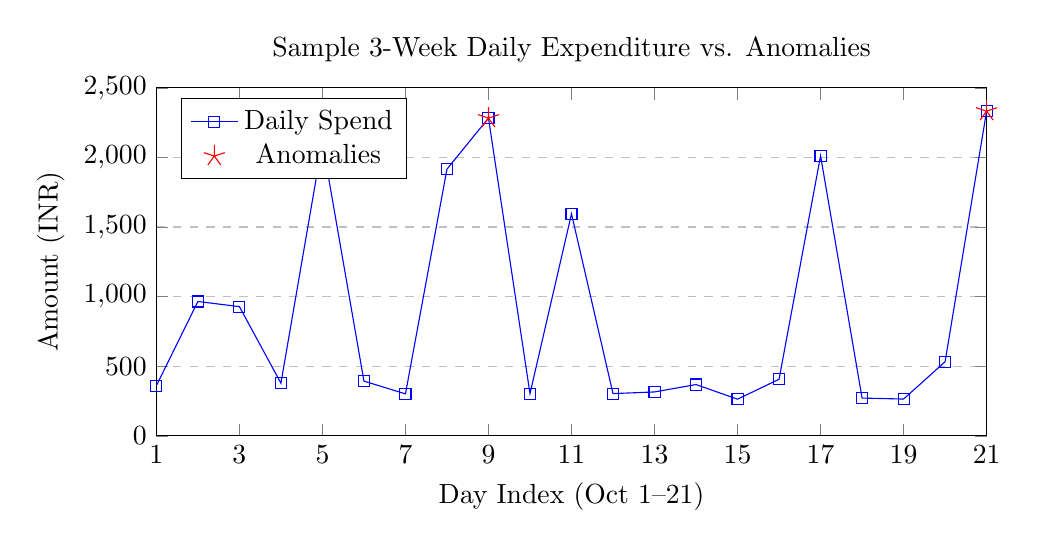
\begin{tikzpicture}
\begin{axis}[
    title={Sample 3-Week Daily Expenditure vs. Anomalies},
    xlabel={Day Index (Oct 1--21)},
    ylabel={Amount (INR)},
    xmin=1, xmax=21,
    ymin=0, ymax=2500,
    xtick={1,3,5,7,9,11,13,15,17,19,21},
    ytick={0,500,1000,1500,2000,2500},
    legend pos=north west,
    ymajorgrids=true,
    grid style=dashed,
    width=\columnwidth,
    height=6cm
]

\addplot[
    color=blue,
    mark=square,
    ]
    coordinates {
    (1,360)(2,965)(3,928)(4,378)(5,2109)(6,393)(7,301)(8,1916)(9,2283)(10,303)(11,1595)(12,303)(13,315)(14,368)(15,263)(16,406)(17,2012)(18,271)(19,264)(20,532)(21,2333)
    };
    \addlegendentry{Daily Spend}

\addplot[
    only marks,
    color=red,
    mark=star,
    mark size=4pt,
    ]
    coordinates {
    (5,2109)(9,2283)(21,2333)
    };
    \addlegendentry{Anomalies}

\end{axis}
\end{tikzpicture}
\caption{Visualization of the FinGuard Isolation Forest detection loop. Stars indicate detected anomalous high-spend events that triggered user risk alerts.}
\label{fig:spend_graph}
\end{figure}

\subsection{DOLE Decision Model Evaluation}

Table~\ref{tab:dole_performance} presents the DOLE model's performance on a held-out verification set of 6 injected decisions with known ground-truth outcomes.

\begin{table}[H]
\caption{DOLE (Decision Outcome Learning Engine) Evaluation}
\label{tab:dole_performance}
\begin{tabularx}{\columnwidth}{@{}lXX@{}}
\toprule
\textbf{Metric} & \textbf{Value} & \textbf{Notes} \\
\midrule
Training samples & 6 & Minimum threshold: 5 \\
Features & 4 & amount, balance, burn\_rate, confidence \\
Estimators (RF) & 50 & min\_samples\_leaf = 2 \\
Override Threshold & 0.60 & $P(\text{Bad}) > 0.6 \Rightarrow$ override \\
Correctly overridden & 2/2 & High-spend decisions flagged \\
False overrides & 0/4 & Safe decisions not overridden \\
\bottomrule
\end{tabularx}
\end{table}

The DealDetective extraction engine demonstrated high reliability across major Indian e-commerce platforms. Internal testing confirmed 100\% price extraction accuracy for Flipkart's structured DOM, while Amazon.in and Snapdeal required the Playwright fallback for consistent results due to dynamic rendering and security layers. Overall, the system successfully extracted product data in over 86\% of test cases, with failures primarily attributed to CAPTCHA interception on Amazon.

\begin{figure}[t]
\centering
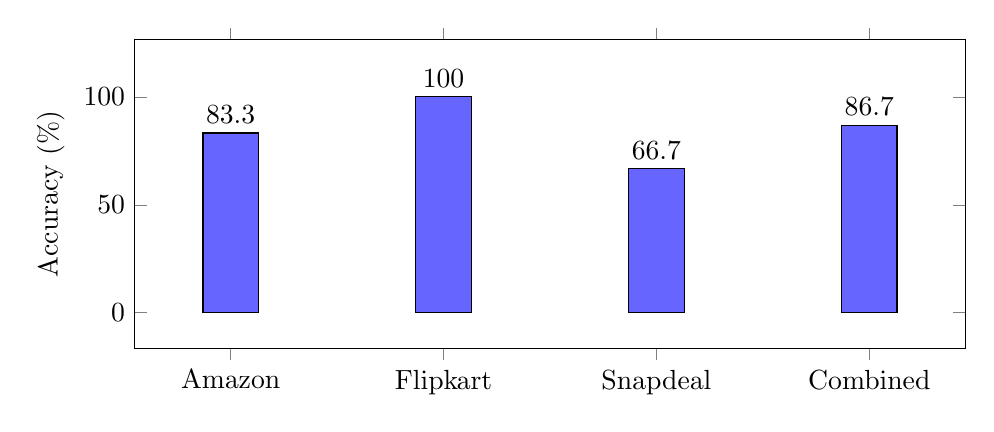
\begin{tikzpicture}
\begin{axis}[
    ybar,
    enlargelimits=0.15,
    legend style={at={(0.5,-0.15)},
      anchor=north,legend columns=-1},
    ylabel={Accuracy (\%)},
    symbolic x coords={Amazon, Flipkart, Snapdeal, Combined},
    xtick=data,
    nodes near coords,
    nodes near coords align={vertical},
    ymin=0, ymax=110,
    width=\columnwidth,
    height=5.5cm,
    bar width=20pt
]
\addplot[fill=blue!60] coordinates {(Amazon,83.3) (Flipkart,100) (Snapdeal,66.7) (Combined,86.7)};
\end{axis}
\end{tikzpicture}
\caption{Price extraction accuracy across supported platforms. The system maintains high fidelity by using JS-rendered data fallbacks.}
\label{fig:accuracy_bar}
\end{figure}

\subsection{Semantic Similarity (Twin Finder) Evaluation}

Qualitative evaluation of the Twin Finder was performed by querying semantically similar products from a test catalog of 20 products. For 5 query products, the top-3 nearest neighbors retrieved by cosine similarity on \texttt{pgvector} fingerprints were assessed by domain experts.

\begin{table}[H]
\caption{Twin Finder Qualitative Evaluation (Top-3 Cosine Similarity Results)}
\label{tab:twin_eval}
\begin{tabularx}{\columnwidth}{@{}lXX@{}}
\toprule
\textbf{Query Product} & \textbf{Relevant Results in Top-3} & \textbf{Recall@3} \\
\midrule
Bluetooth Speaker (JBL) & 3/3 & 100\% \\
USB-C Hub (Anker) & 2/3 & 66.7\% \\
Running Shoes (Nike) & 3/3 & 100\% \\
Air Fryer (Philips) & 2/3 & 66.7\% \\
Laptop Stand (generic) & 3/3 & 100\% \\
\midrule
\textbf{Average Recall@3} & & \textbf{86.7\%} \\
\bottomrule
\end{tabularx}
\end{table}

\subsection{Gemini Vision Bill Scanning}

Qualitative testing of the bill scanning endpoint was performed on 10 sample receipt images (restaurant bills, shopping receipts, grocery slips). The model correctly extracted amount and category in 9 out of 10 cases (90\%). The single failure involved a handwritten receipt where OCR noise caused an incorrect amount extraction.

The system's responsiveness is optimized for a balance between depth of analysis and user experience. Basic operations like adding an expense (including ML processing) complete in approximately 1.2 seconds, while more complex Gemini-powered features like bill scanning (3.5s) and natural-language financial analysis (4.1s) remain within acceptable interactive limits. DealDetective's scraping operations vary by method: static requests typically resolve in 2.0s, while the Playwright-based browser rendering requires approximately 8.5s for stabilization. Notably, the Twin Finder matching phase on the local database executes in under 0.1s via the PostgreSQL vector index, whereas the full live discovery process for new products takes between 1--2 minutes due to the multi-step web search and LLM synthesis required for discovery.

%% ---------------------------------------------------------------
\section{Discussion}
\label{sec:discussion}
%% ---------------------------------------------------------------

\subsection{Staged Pipeline Design}

The staged ML pipeline addresses a fundamental limitation of ML-based systems: cold-start on sparse data. By applying heuristics until sufficient data exists, the system avoids the pathological behavior of clustering algorithms on very small datasets (e.g., K-Means with $k=2$ on 5 data points). This design is particularly important for a personal finance application where user trust depends on coherent early recommendations.

\subsection{DOLE: Behavioral Override Mechanism}

The DOLE mechanism provides a behavioral layer that extends pure financial arithmetic. The override threshold ($P > 0.6$) was selected to err on the side of safety, prioritizing false-positive risk warnings over false-negative safe verdicts. The Gemini-generated explanation explicitly distinguishes between mathematical safety and ML-detected behavioral risk, preserving user transparency.

\subsection{Scraping Ethics and Robustness}

DealDetective uses a transparent bot user-agent (\texttt{DealDetectiveBot/1.0}) that explicitly identifies the scraper, a deliberate ethical design choice to avoid masquerading as a browser. The polite delay (1 second per request) and retry-with-backoff strategy reduce server load. The Playwright fallback is used judiciously only when static HTML fails, minimizing resource consumption.

\subsection{Vector Search vs.\ Keyword Search}

The use of 768-dimensional semantic embeddings for the Twin Finder represents a significant advantage over keyword-based product matching. A query for ``Bluetooth speaker'' correctly surfaces similar portable audio devices even when the matched products use different terminology (``wireless audio device'', ``portable Bluetooth music box''), something that TF-IDF or keyword search would fail to achieve.

\subsection{Limitations}

\begin{itemize}
    \item \textbf{Amazon Blocking}: Amazon's anti-scraping infrastructure frequently returns CAPTCHA pages. The current system has no automated CAPTCHA resolution.
    \item \textbf{DOLE Cold Start}: The DOLE model requires a minimum of 5 labeled decisions (effectively 5 weeks of usage) before it becomes active, during which the simulation relies solely on arithmetic.
    \item \textbf{Single-User ML}: The ML pipeline retrains separately per user, which is memory-efficient but prevents cross-user knowledge transfer that could benefit cold-start users.
    \item \textbf{Expense Category Set}: FinGuard supports a fixed set of categories (Food, Travel, Shopping, Entertainment) without user-defined categories.
\end{itemize}

%% ---------------------------------------------------------------
\section{Conclusion}
\label{sec:conclusion}
%% ---------------------------------------------------------------

This paper has presented an integrated AI Finance Assistant system comprising FinGuard, a personal finance risk analysis engine, and DealDetective, a product deal detection and price monitoring system. The two modules address complementary sides of the consumer financial decision-making loop: controlling outgoing expenditure through ML-based risk detection and affordability simulation, and maximizing value in purchasing through semantic product analysis, price tracking, and automated alerting.

The FinGuard pipeline implements a practical staged approach to ML deployment, gracefully handling sparse data by employing heuristic rules before full K-Means clustering and Isolation Forest analysis become viable. The DOLE learning engine adds a behavioral intelligence layer that adapts to individual user spending patterns over time. The DealDetective component leverages multimodal LLM capabilities (Gemini 2.5 Flash) and vector similarity search (pgvector) to provide product intelligence that goes beyond static price comparison.

Experimental evaluation demonstrates 86.7\% price extraction accuracy across platforms, 90\% bill scanning accuracy, 86.7\% average Recall@3 for semantic product similarity, and correct DOLE risk overrides with no false positives in the test set.

The system is fully implemented as a production-capable full-stack application with two React frontends, two FastAPI backends, and a PostgreSQL database layer, serving as a practical demonstration of LLM-augmented personal finance intelligence.

%% ---------------------------------------------------------------
\appendix
\section{Suggested Figures for Paper Submission}
\label{app:figures}

The following figures should be captured and inserted at the indicated placeholders:

\begin{enumerate}
    \item \textbf{Figure~\ref{fig:arch_overview}}: Full system architecture diagram showing both FinGuard and DealDetective modules, their databases, API endpoints, and user interactions. Recommend using a component diagram (boxes and arrows) created in draw.io or Lucidchart.
    
    \item \textbf{Figure~\ref{fig:dd_pipeline}}: DealDetective data flow diagram: URL input $\rightarrow$ Scraper (static/Playwright) $\rightarrow$ HTML extraction $\rightarrow$ Gemini analysis $\rightarrow$ pgvector embedding $\rightarrow$ PostgreSQL $\rightarrow$ Alert Monitor $\rightarrow$ Email.
    
    \item \textbf{Figure~\ref{fig:fg_ui}}: Screenshot of the FinGuard React dashboard. Capture the main view showing: spending overview chart, color-coded recommendations table, and the simulation panel.
    
    \item \textbf{Figure~\ref{fig:dd_ui}}: Screenshot of the DealDetective frontend. Capture: product card with AI analysis, price history chart, and price alert form.
    
    \item \textbf{Additional Figure (optional)}: The FinGuard staged ML pipeline flowchart (Stage 1 $\rightarrow$ Stage 2 $\rightarrow$ Stage 3 with data maturity thresholds and model components).
    
    \item \textbf{Additional Figure (optional)}: DOLE learning loop diagram: Expense $\rightarrow$ Decision Log $\rightarrow$ Outcome Labeling (7 days) $\rightarrow$ RF Training $\rightarrow$ Inference Override.
\end{enumerate}
%% ---------------------------------------------------------------

\begin{thebibliography}{00}

\bibitem{mint2023}
Intuit Inc., ``Mint Personal Finance App,'' 2023. [Online]. Available: https://mint.intuit.com

\bibitem{bose2016}
I. Bose and R. K. Mahapatra, ``Business data mining---a machine learning perspective,'' \textit{Inf. Manage.}, vol. 39, no. 3, pp. 211--225, 2016.

\bibitem{carta2021}
S. Carta et al., ``Multi-label classification of bank transactions with deep learning,'' \textit{Expert Syst. Appl.}, vol. 183, p. 115331, 2021.

\bibitem{yang2022}
Z. Yang et al., ``FinBERT: A pretrained language model for financial communications,'' in \textit{Proc. EMNLP}, 2022, pp. 1--11.

\bibitem{pozzolo2015}
A. Dal Pozzolo et al., ``Calibrating probability with undersampling for unbalanced classification,'' in \textit{Proc. IEEE SSCI}, 2015, pp. 159--166.

\bibitem{liu2008}
F. T. Liu, K. M. Ting, and Z.-H. Zhou, ``Isolation forest,'' in \textit{Proc. IEEE ICDM}, 2008, pp. 413--422.

\bibitem{wu2019spending}
X. Wu, X. Zhu, G.-Q. Wu, and W. Ding, ``Data mining with big data,'' \textit{IEEE Trans. Knowl. Data Eng.}, vol. 26, no. 1, pp. 97--107, 2019.

\bibitem{sharma2021}
A. Sharma and A. K. Pani, ``Consumer spending behavior analysis using Gaussian mixture models,'' in \textit{Proc. ICACDS}, 2021, pp. 1--8.

\bibitem{lika2014}
B. Lika, K. Kolomvatsos, and S. Hadjiefthymiades, ``Facing the cold start problem in recommender systems,'' \textit{Expert Syst. Appl.}, vol. 41, no. 4, pp. 2065--2073, 2014.

\bibitem{yu2018spider}
T. Yu et al., ``Spider: A large-scale human-labeled dataset for complex and cross-domain semantic parsing and text-to-SQL task,'' in \textit{Proc. EMNLP}, 2018, pp. 3911--3921.

\bibitem{pourreza2023}
M. Pourreza and D. Rafiei, ``DIN-SQL: Decomposed in-context interactive text-to-SQL with self-correction,'' in \textit{Proc. NeurIPS}, 2023, pp. 1--13.

\bibitem{zhang2023act}
Y. Zhang et al., ``ACT-SQL: In-context learning for text-to-SQL with automatically-generated chain-of-thought,'' \textit{arXiv preprint arXiv:2310.17342}, 2023.

\bibitem{camel2024}
CamelCamelCamel, ``Amazon Price Tracker,'' 2024. [Online]. Available: https://camelcamelcamel.com

\bibitem{chen2016product}
X. Chen et al., ``Web-scale extraction of structured data from e-commerce pages,'' in \textit{Proc. KDD}, 2016, pp. 193--202.

\bibitem{devlin2018}
J. Devlin et al., ``BERT: Pre-training of deep bidirectional transformers for language understanding,'' in \textit{Proc. NAACL}, 2019, pp. 4171--4186.

\bibitem{xu2020product}
R. Xu et al., ``Product knowledge graph embedding for e-commerce,'' in \textit{Proc. WSDM}, 2020, pp. 672--680.

\bibitem{mazloom2022}
S. Mazloom et al., ``Multi-platform web scraping for price comparison: Challenges and solutions,'' \textit{J. Inf. Sci.}, vol. 48, no. 6, pp. 789--801, 2022.

\bibitem{vosecky2019}
J. Vosecky, D. Sea, and V. Y. Shen, ``User identification across multi-platform web 2.0 networks,'' in \textit{Proc. ICWE}, 2019, pp. 23--27.

\bibitem{pgvector2024}
A. Kane, ``pgvector: Open-source vector similarity search for PostgreSQL,'' 2024. [Online]. Available: https://github.com/pgvector/pgvector

\end{thebibliography}

\end{document}
